\section{Task Decomposition}

Modularization is one approach to reduce the dimension of the state space. In
this section, we will discuss some major approaches of MDP decomposition as
solutions to the curse of dimensionality, and analyze their similarity and
difference compared to the modular approach. We will discuss a hierarchical
approach and a layered approach.

Some complex tasks have explicit phases. Take the taxi domain for example
(Figure~\ref{fig:taxi}). The taxi driver picks up a passenger from a location,
and drives and drops him at a different location. This task requires some shared
low-level skills.

\begin{figure}[h]
\centering
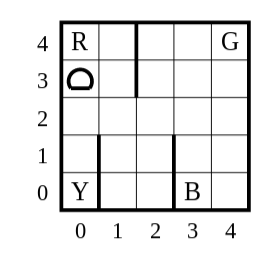
\includegraphics[width=0.3\textwidth]{taxi.png}
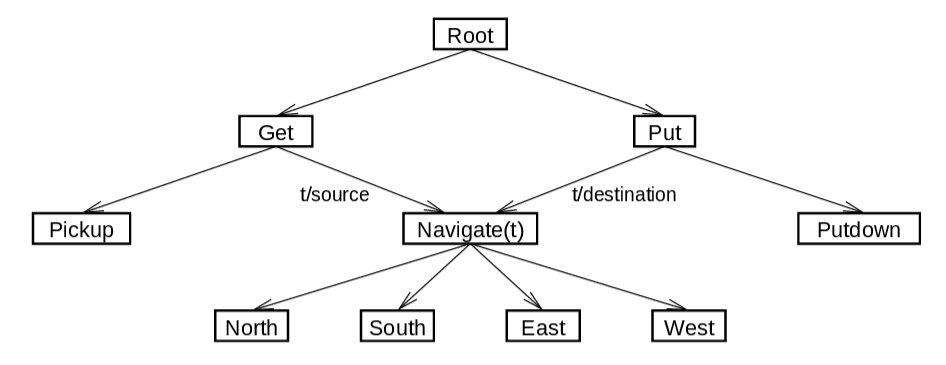
\includegraphics[width=0.6\textwidth]{maxq.png}
\caption{(Left) Taxi domain. (Right) A decomposition of the task.}
\label{fig:taxi}
\end{figure}

This is generally known as hierarchical reinforcement learning (hierarchical RL)
\cite{dietterich2000hierarchical}.
We assume that there is a known structure of the task, and the
learning is decomposed hierarchically. At a higher level, an action can be
which lower level task to execute. For example, in the Get task, the two actions
available would be Pickup and Navigate. At the bottom level, primary actions are
available.

A similar approach is skill chaining \cite{konidaris2009skill}, which can
be seen as a hierarchical RL approach. Figure~\ref{fig:skills} shows
an example that a robot navigates in a domain with obsacles. The red circle is
the goal. The robot starts from the left-bottom corner. It has several trained
skills, represented by different colors. The robot learns which skill to use,
and when to terminate and switch to another skill.

\begin{figure}[h]
\centering
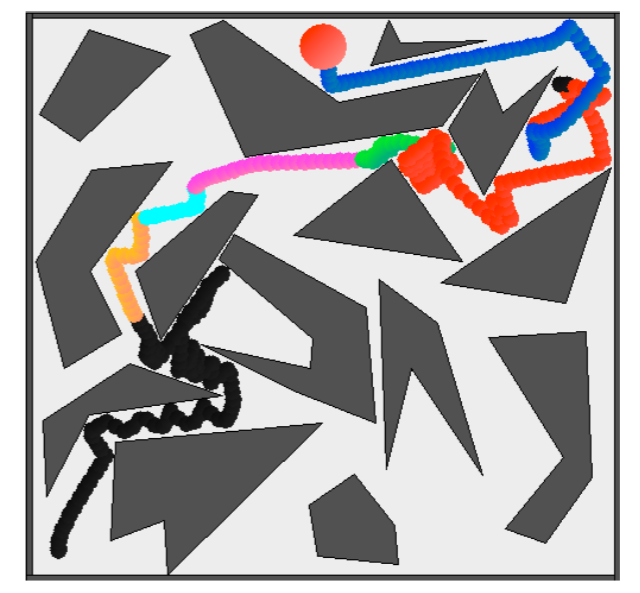
\includegraphics[width=0.5\textwidth]{skills}
\caption{(Left) Taxi domain. (Right) A decomposition of the task.}
\label{fig:skills}
\end{figure}

Hierarchical reinforcement learning is different from modular reinforcement
learning in a way that the former approach doesn't involve concurrent modules
(or sutasks, skills, depending on context).
For example, the Pickup module doesn't run parallel with Navigate module.
Therefore, there is no compromise in policies proposed by different modules.

Apart from hierachical RL, layered learning is another approach to decompose a
complex task \cite{stone2000layered}. This is a general learning method that may
not restricted to reinforcement learning. Similar to hierarchical learning, it
also assumes a hierarchy of the task. A module has some parameters. When one
layer is optimized, the upper layer.

Layered learning is similar to modular reinforcement learning, as the modules are
run in parallel. However different modules correspond to different controllers
or agents. They need to compromise to contribute to a higher level module, but
not sharing a single controller.
A recent work in layered learning makes some parameters in lower level modules
available to change in the process of training of a higher level module
\cite{macalpine2015ut}. This is the same idea as parameterizing modules in
modular reinforcement learning. 

\section{Inverse Reinforcement Learning}

We introduced basic concepts of inverse reinforcement learing in the last
chapter. In this section, we discuss some advances in IRL and compare them with
our methods.

The original IRL algorithm is formulated by
\cite{abbeel2004apprenticeship,ng2000algorithms}. A popular following work is
Bayesian inverse reinforcement learning (Bayesian IRL) \cite{ramachandran2007bayesian}.
It is motiviated by the
observation that rewards are not completely arbitrary. We can reasonably assume
some prior knowledge of the rewards. Bayesian IRL assumes that the rewards are
drawn from a prior distribution. 
For example, in most of the problems, rewards are generally sparse. So the
reward of a state is very likely to be 0. A Gaussian or Laplacian prior can be
applied.  In planning problems, on the contrary, rewards are generally small but
positive for most of the states. Then a Beta prior can be applied.

Other recent developments in Bayesian IRL include
\cite{choi2011map,choi2012nonparametric,dimitrakakis2012bayesian}.
\cite{choi2011map} uses MAP inference to solve the Bayesian IRL problem.
\cite{choi2012nonparametric,dimitrakakis2012bayesian} tackle the problem of
recovering rewards in domains with multiple tasks or multiple rewards. 
